% !TeX root = ../main.tex
\section{Generation 3: look-ahead never leads}
\label{sec:gen3}

Generation~3 is the instrumented rebuild: bf16 generation, eight evaluation instruments,
persona-level pairing, measured oracle reproducibility, and every conversation re-scored by a
second grader from a different model family. Its PTO look-ahead arm reaches eight matched
iterations against the myopic arm.

\begin{table}[t]
\centering\small
\begin{tabular}{@{}lrrrrrr@{}}
\toprule
\textbf{Iter.} & \multicolumn{3}{c}{\textbf{\primaryjudge{}} (primary)} & \multicolumn{2}{c}{\textbf{\heldout{}} (held out)} \\
\cmidrule(lr){2-4}\cmidrule(lr){5-6}
 & $\K{=}0$ & $\K{=}5$ & $\dlt$ & $\dlt$ & $\dz$ \\
\midrule
1 & 3.264 & 3.181 & $+0.083$ & $+0.060$ & $+0.09$ \\
2 & 3.466 & 3.308 & $+0.158$ & $+0.136$ & $+0.20$ \\
3 & 3.815 & 3.674 & $+0.141$ & $+0.130$ & $+0.20$ \\
4 & 4.008 & 3.888 & $+0.120$ & $+0.123$ & $+0.21$ \\
5 & 4.014 & 4.017 & $-0.002$ & $+0.173^{*}$ & $+0.33$ \\
6 & 4.154 & 3.897 & $+0.257^{*}$ & $+0.343^{*}$ & $+0.51$ \\
7 & 4.129 & 4.085 & $+0.044$ & $+0.078$ & $+0.12$ \\
8 & 4.221 & 4.144 & $+0.077$ & $+0.186^{*}$ & $+0.34$ \\
\midrule
mean & & & $\mathbf{+0.110}$ & $\mathbf{+0.154}$ & \\
\bottomrule
\end{tabular}
\caption{Generation~3, PTO. $\dlt = \K_0 - \K_5$ on \QQ{}, persona-paired, $n = 96$ per cell;
\emph{positive} means look-ahead \textbf{cost} score. $^{*}$ Holm-corrected $p < 0.05$. The
primary oracle's iteration-5 value ($-0.002$) is a dead heat, not a lead. Held-out-judge values
for iterations 5, 6 and 8 are Holm-significant \emph{against} look-ahead.}
\label{tab:gen3}
\end{table}

\subsection{The result}
Across eight matched iterations, \textbf{look-ahead never leads}. Under the primary oracle the
sign favours $\K{=}0$ at seven of eight iterations; the eighth (iteration~5,
$\dlt = -0.002$, $\dz = -0.004$) is a dead heat rather than a win. One iteration reaches
significance and it favours the \emph{absence} of look-ahead: iteration~6, $\dlt = +0.257$,
$\dz = 0.42$, Holm $p < 0.001$. At the arm's configured endpoint (iteration~8) the myopic arm
leads $4.221$ to $4.144$.

\subsection{The held-out grader agrees, and is less generous}
Every conversation was independently re-scored by \heldout{}, a grader from a different model
family that never played the patient and never touched training. It puts $\K{=}0$ ahead at
\textbf{every} one of the eight iterations, with a larger mean gap ($+0.154$ versus $+0.110$)
and three Holm-significant cells (iterations~5, 6 and~8) against look-ahead's zero.

The two graders therefore agree on the conclusion and disagree only on its generosity. That
disagreement is itself informative and worth stating precisely, because an earlier reading of
this arm --- based on the primary oracle alone and on five iterations --- concluded that the
arms ``converge at iteration~5''. They do not. The convergence was a single primary-oracle
data point that the held-out judge never saw as a tie ($+0.173$, $\dz = 0.33$, Holm
$p = 0.017$) and that did not survive the next iteration. \textbf{The claim that survives both
graders and all eight iterations is about the lever --- $\K{=}5$ never wins --- not about
convergence.}

\subsection{A signal that does not hold up}

\paragraph{An MI-consistency tilt.}
At iterations~2--5, both graders showed the $\K{=}5$ arm producing \emph{more} MI-inconsistent
behaviour --- significantly so at iteration~4 under both ($-0.111$ primary, $-0.177$ held-out).
That looked like evidence that look-ahead trades MI fidelity for questionnaire score. It does
not survive the longer run: at iterations~7 and~8 the sign reverses and $\K{=}5$ becomes the
more MI-consistent arm ($+0.078$ and $+0.059$ primary, $+0.071$ held-out at iteration~8, all
Holm-significant or near it). A contrast that changes sign partway through a run is a statement
about \emph{when}, not about the lever, so we record it as unresolved and draw no conclusion
from it. It is mentioned here because it was a live hypothesis in earlier drafts of this work
and readers of those drafts should know it was withdrawn on further data.

\subsection{Summary across the three generations}
Figure~\ref{fig:trajectories} shows all three trajectories on the common grader, and
Table~\ref{tab:headline} collects the contrasts.

\begin{table}[t]
\centering\small
\begin{tabular}{@{}lrrrrl@{}}
\toprule
\textbf{Generation} & \textbf{Contrasts} & $\K{=}5$ \textbf{ahead} & \textbf{mean} $\dlt$ & \textbf{mean} $\dz$ & \textbf{Verdict} \\
\midrule
1 --- Llama-2-7B       & 7  & $7/7$  & $-0.132$ & $-0.18$ & look-ahead helps \\
2 --- Llama-3.2-1B (4-bit) & 15 & $9/15$ & $-0.019$ & $-0.02$ & null \\
3 --- Llama-3.2-1B (bf16)  & 8  & $1/8$  & $+0.110$ & $+0.17$ & never leads \\
\bottomrule
\end{tabular}
\caption{The three generations on one measurement axis (\primaryjudge{}, \QQ{},
persona-paired). $\dlt = \K_0 - \K_5$; negative favours look-ahead. Generation~2's $15$
contrasts are $3$ training oracles $\times$ $5$ iterations. Generation~3's single ``ahead'' cell
is the $-0.002$ dead heat at iteration~5.}
\label{tab:headline}
\end{table}

\begin{figure}[t]
\centering
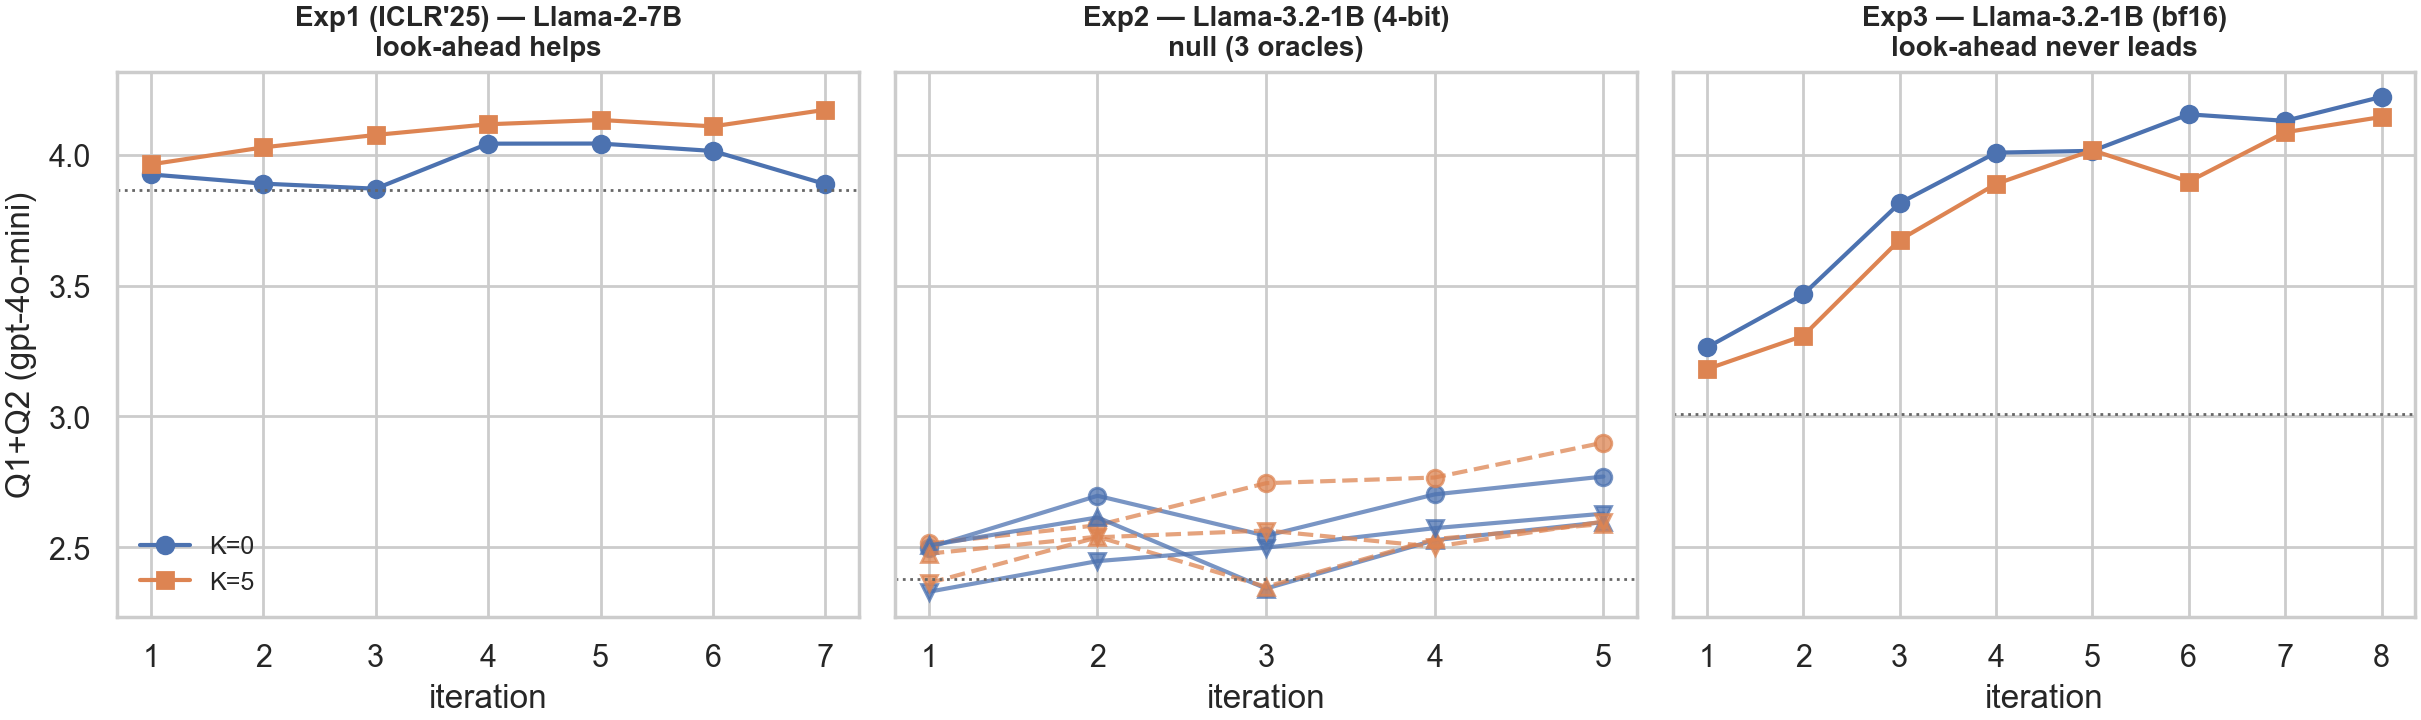
\includegraphics[width=\linewidth]{figures/fig1_trajectories.png}
\caption{\QQ{} per iteration, all three generations under the same \primaryjudge{} grader.
Dotted lines mark each generation's untrained base. Left: look-ahead (orange) separates from the
myopic arm (blue), which tracks its base for all seven iterations. Middle: three training
oracles, arms tangled. Right: the myopic arm leads throughout. Absolute levels are not
comparable across panels (\S\ref{sec:generations}); the within-panel gap is the result.}
\label{fig:trajectories}
\end{figure}
